\clearpage
\setcounter{page}{1}
\maketitlesupplementary

We include here all the hyperparameters used in the experiments presented in the main paper, together with more qualitative visualisations of  results for the point tracking task (section~\ref{sec:mae}) and the long video memorisation task (section~\ref{sec:longtask}). Videos showing point tracks are also attached. 

\section{Training hyperparameters}
\label{sec:hyper}

\subsection{Supervised video classification}

\begin{table}[h!]
    \centering
    \begin{tabular}{l|c|c}
     \textbf{Hyperparameter} & \textbf{Kinetics400} & \textbf{SSv2} \\
     \hline
      Peak learning rate  & 1e-4 & 1e-4 \\
      Weight decay & 0.03 & 0.03 \\
      Label smoothing & 0.1 & 0.1 \\
      Scale jitter & (0.875, 1.33) & (0.875, 1.33) \\
    %   Colour jitter & & \\
      Num frames & 32 & 32 \\
      Stride & 2 & 2 \\
      Cls dropout & - & 0.1 \\
      Rand augment & - & yes \\
    %   Cropping &  & \\
      Epochs & 30 & 35 \\
      Spatial crops eval & 3 & 3 \\
      Temporal clips eval & 4 & 4\\
      \hline
    \end{tabular}
    \caption{Hyperparameter values used in the supervised classification experiments. These are mainly the hyperparameters used in previous works, \eg ViViT~\cite{vivit}. For both datasets, we use cosine decay for the learning rate schedule with linear warmup.}
    \label{tab:hyperssup}
\end{table}

\subsection{Self-supervised masked autoencoding and fine-tuning}

\begin{table}[h!]
    \centering
    \begin{tabular}{l|c}
     \textbf{Hyperparameter} & \textbf{Kinetics400} \\
     \hline
      Learning rate  & 3e-4  \\
      Weight decay & 0.05 \\
      Num frames & 16  \\
      Stride & 2  \\
      Epochs & 1600  \\
      Mask ratio & 0.9 \\
      \hline
    \end{tabular}
    \caption{Hyperparameter values used in the self-supervised masked auto-encoding experiment on Kinetics400. We use AdamW optimizer. We apply patch-wise normalisation of the inputs as done in VideoMAE~\cite{tong2022videomae}}
    \label{tab:hypersssup}
\end{table}

\begin{table}[h!]
    \centering
    \begin{tabular}{l|c|c}
     \textbf{Hyperparameter} & \textbf{Kinetics400} & \textbf{SSv2} \\
     \hline
      Learning rate  & 3e-4 & 3e-4 \\
      Scale jitter & (0.9, 1.33) & (0.9, 1.33) \\
    %   Colour jitter & & \\
      Num frames & 16 & 16 \\
      Stride & 2 & 2 \\
      Epochs & 30 & 6 \\
      Spatial crops eval & 3 & 3 \\
      Temporal clips eval & 4 & 4\\
      \hline
    \end{tabular}
    \caption{Hyperparameter values used in the fine-tuning classification experiments. We use cosine decay for the learning rate schedule with 1k steps of linear warmup.}
    \label{tab:hypersFTcls}
\end{table}

\begin{table}[h!]
    \centering
    \begin{tabular}{l|c|c}
     \textbf{Hyperparameter} & \textbf{DAVIS} & \textbf{Perception Test} \\
     \hline
      Learning rate  & 3e-4 & 3e-4 \\
      Num frames & 8 & 16 \\
      Num steps & 200k & 40k \\
      \hline
    \end{tabular}
    \caption{Hyperparameter values used in the point tracking fine-tuning experiments. We use cosine decay for the learning rate schedule with 1k steps of linear warmup.}
    \label{tab:hypersFTpt}
\end{table}

\section{Point tracking qualitative results}

In Figure~\ref{fig:supmattracking}, we include more visualisations for the point tracking task using frozen MAE representations pre-trained on Kinetics400, using \ssm\ as backbone.  

 \begin{figure*}[h]
  \centering
    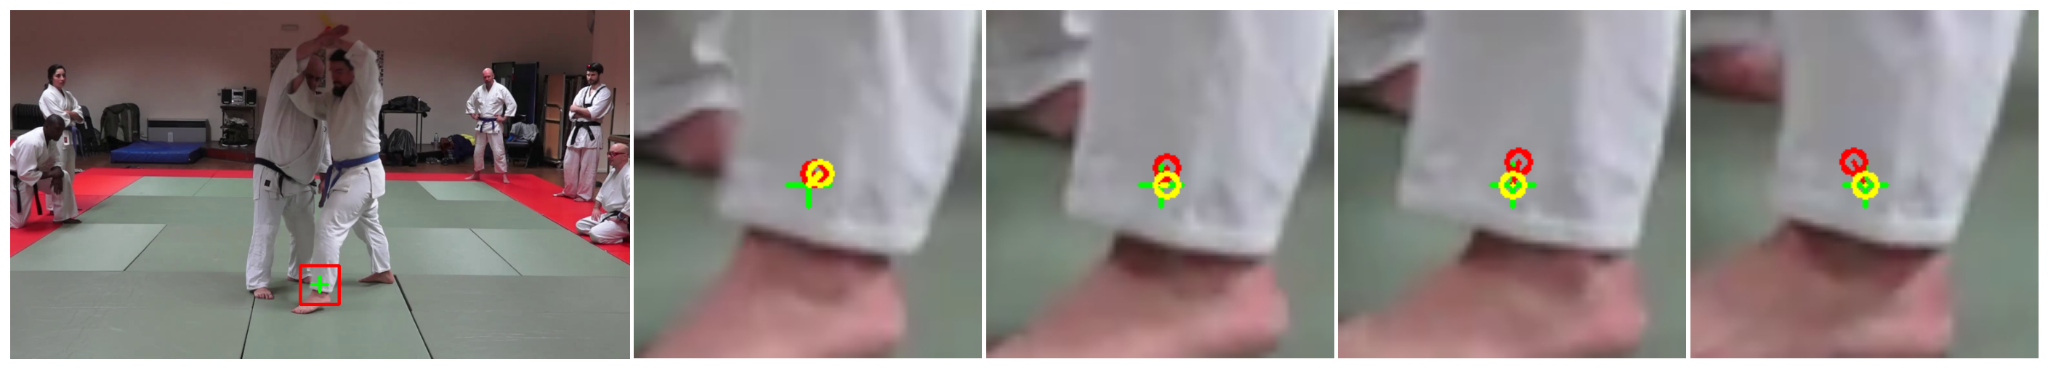
\includegraphics[width=\linewidth]{img/leg.png}
    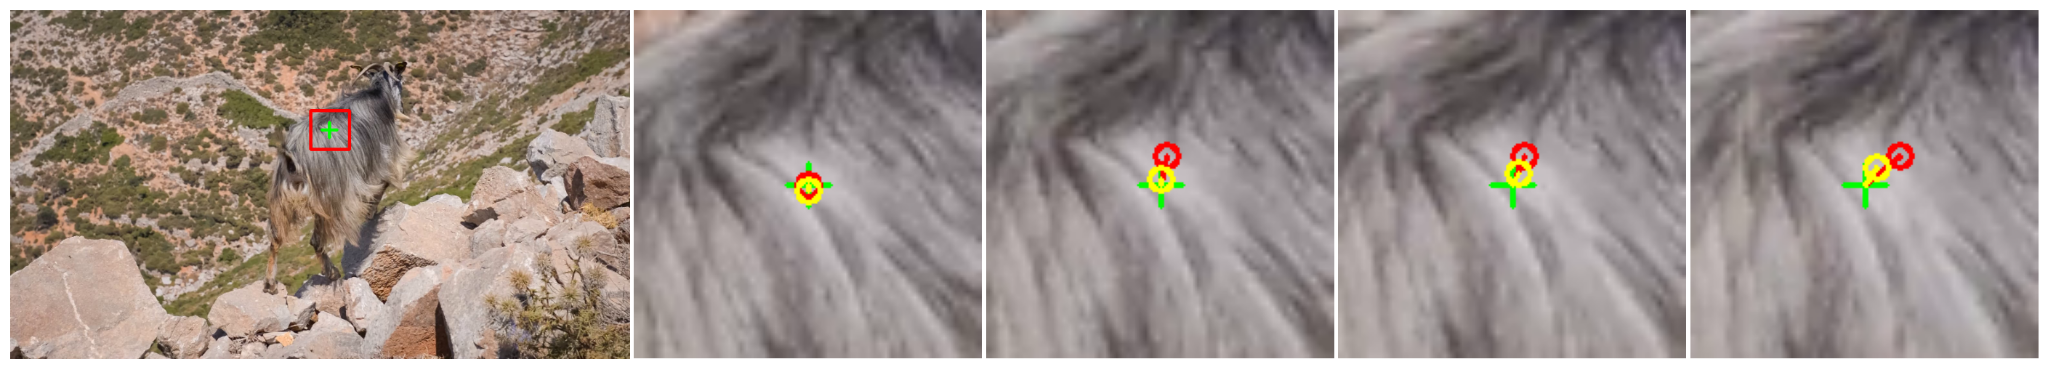
\includegraphics[width=\linewidth]{img/goat.png}
    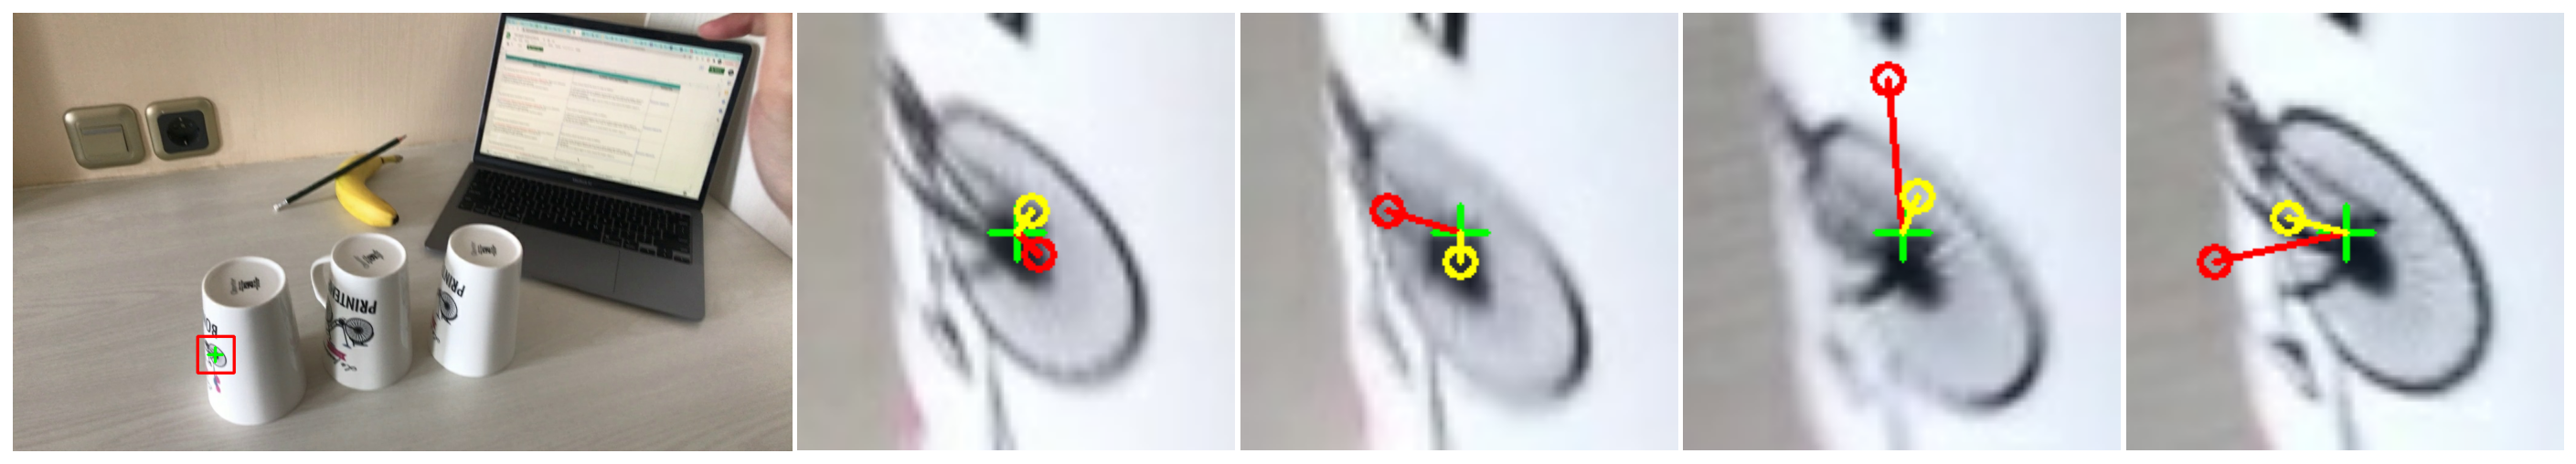
\includegraphics[width=\linewidth]{img/ptbike.png}
    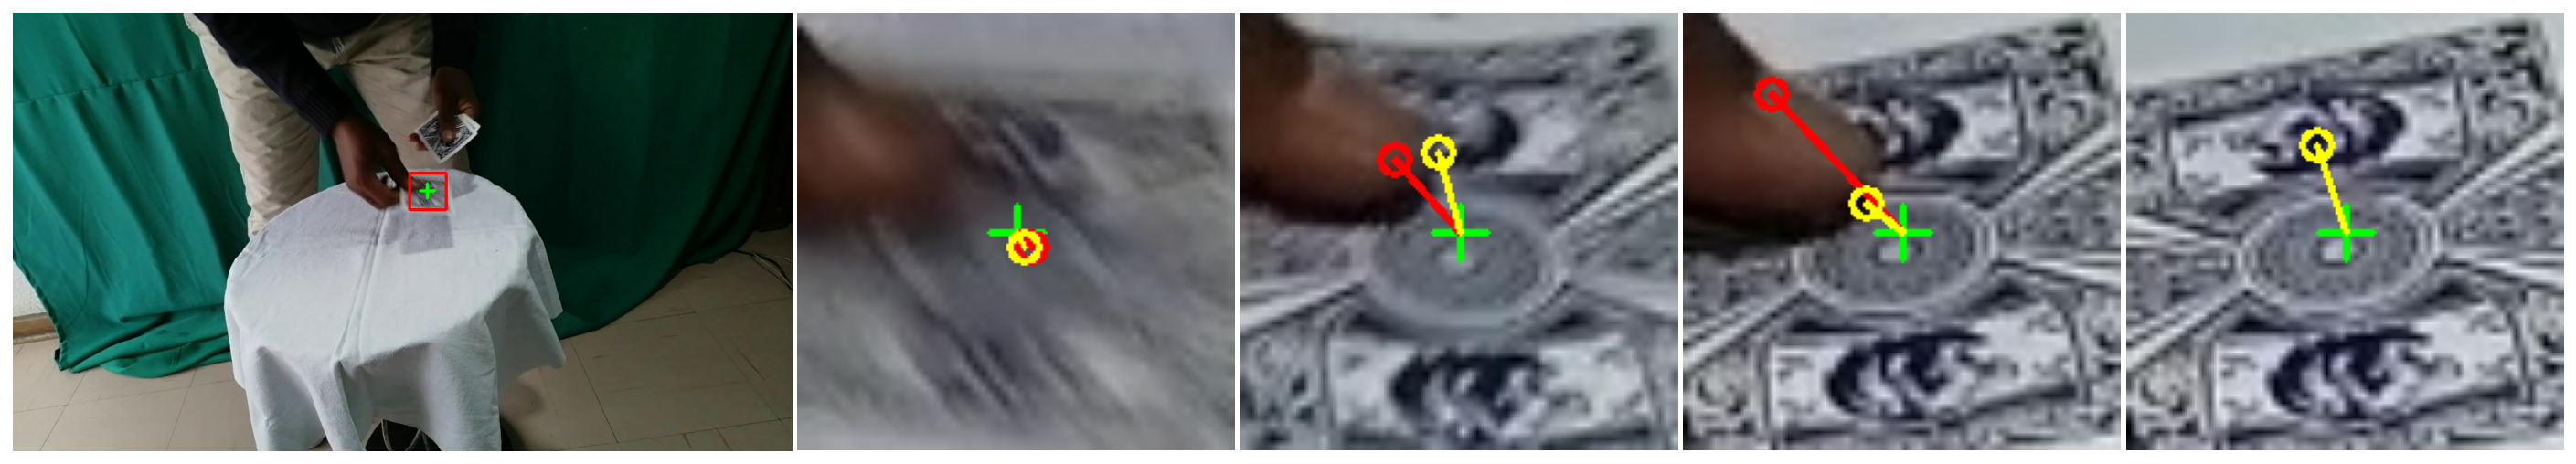
\includegraphics[width=\linewidth]{img/ptcard.png}
    
  \caption{Qualitative results obtained by \ssm\ for point tracking on DAVIS dataset (rows 1-2) and Perception Test (rows 3-4) compared to VideoMAE. The leftmost image indicates the point to track in the original frame, and the images towards the right show zoom-ins on subsequent frames. Green plus (+) marker indicates the ground truth, yellow circle indicates \ssm's predictions and red circles indicate VideoMAE's predictions.}
  \label{fig:supmattracking}
\end{figure*}

\section{Long video memorisation task}

Figure~\ref{fig:supmatmem} shows qualitative results for the memorisation task. For easier visual comparison, we increase the distance $k$ to the frame to reconstruct while also increasing the video length $T$, so the frame to reconstruct is always the same. For ViViT-L (3rd row), the quality of the reconstruction is very good and does not degrade as $k$ increases. However, the model goes out-of-memory for $T>96$. For \ssm, the high frequencies are less well reconstructed as $k$ increases, but overall the model is able to perform the task reasonably well even at $T=160,k=144$, \ie it is able to learn with sequences of up to 5.3s long at 30FPS, and remember a frame seen about 4.8s before.  

\begin{figure*}[h]
  \centering
    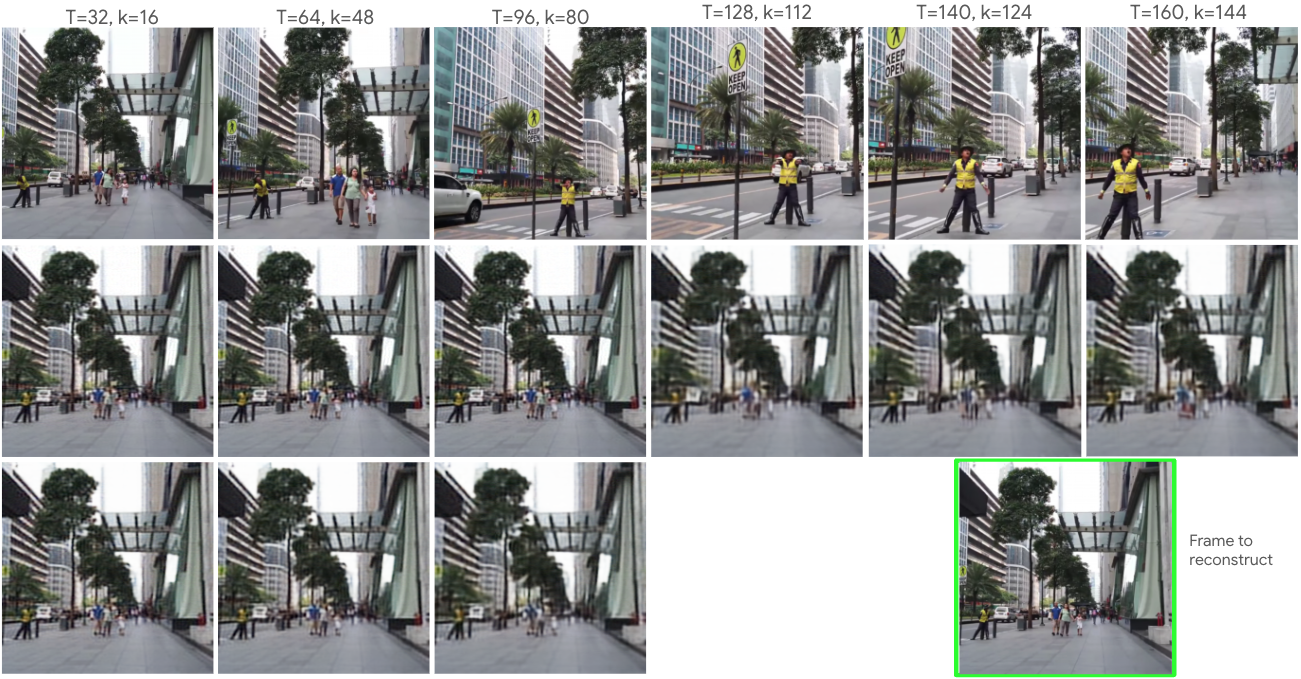
\includegraphics[width=\linewidth]{img/longtaskmany.png}
    
  \caption{Qualitative results for the task of reconstructing a frame from the past, for increasing distance $k$ to the frame to reconstruct from left to right. \textbf{First row}: last frame seen by the model. \textbf{Second row}: \ssm\ output. \textbf{Third row}: ViViT-L output; ViViT-L goes OOM for $k>80$, so no predictions are shown.}
  \label{fig:supmatmem}
\end{figure*}
